\chapter{Problem definition}
\section{Foreword}
The second course used for the semester project is Procedural Programming, in which programming skills in C++ are learned. The theoretical background for programming is necessary to complete image manipulations, based on methods learned in Image Processing.

The eleven subjects presented was:

\begin{itemize}
\item Image Processing for Fun Utilizing an Industrial Robot
\item Image Processing for Ambient Intelligent Robots
\item Interactive Floor
\item Interactive Book
\item Interactive Drawing Game
\item Interactive Arcade Game
\item Emergency system for old people that have fallen
\item Thermal Sock Puppet Show
\item Body Motion Controlled Exercise Game
\item Hjørring Library
\end{itemize}

\section{Establishing collaboration with Hjørring Library}

As only three groups on the third semester applied for working with Hjørring Library, our group was chosen. A meeting was arranged with Hjørring Library and so together with 5 other groups from third and fifth semester of Medialogy, all groups travelled to Hjørring to meet the library staff. In addition the groups were let loose in the library to check locations for potential projects.\\
After talking to some of the staff, more specific our contact person Martin Jørgensen, some general ideas emerged, so it was decided to go back to the group room at Novi to do some brainstorming within the group.


After conferencing with the supervisor, Thomas Moeslund, and the co-supervisor, Andreas Møgelmose, it was decided that the conceptual idea needed to be narrowed down to a more specific subject field. The second idea emerged that we should focus mainly on fairy tales and first of all work around H.C. Andersen, which meant adding a hat on-top of the users.


\begin{itemize}
\item The position of the project
\item The equipment that was desired to borrow
\item The light conditions
\end{itemize}

The position of the project will be on the walkway from the reception desk to the core of the library, which Martin believed would be an ideal position for the project, as the light conditions are controllable. In addition to that he knew from experience that people tend to use that walkway either to enter or exit the library, as it is the shortest route.

\begin{figure}[htbp]
\centering
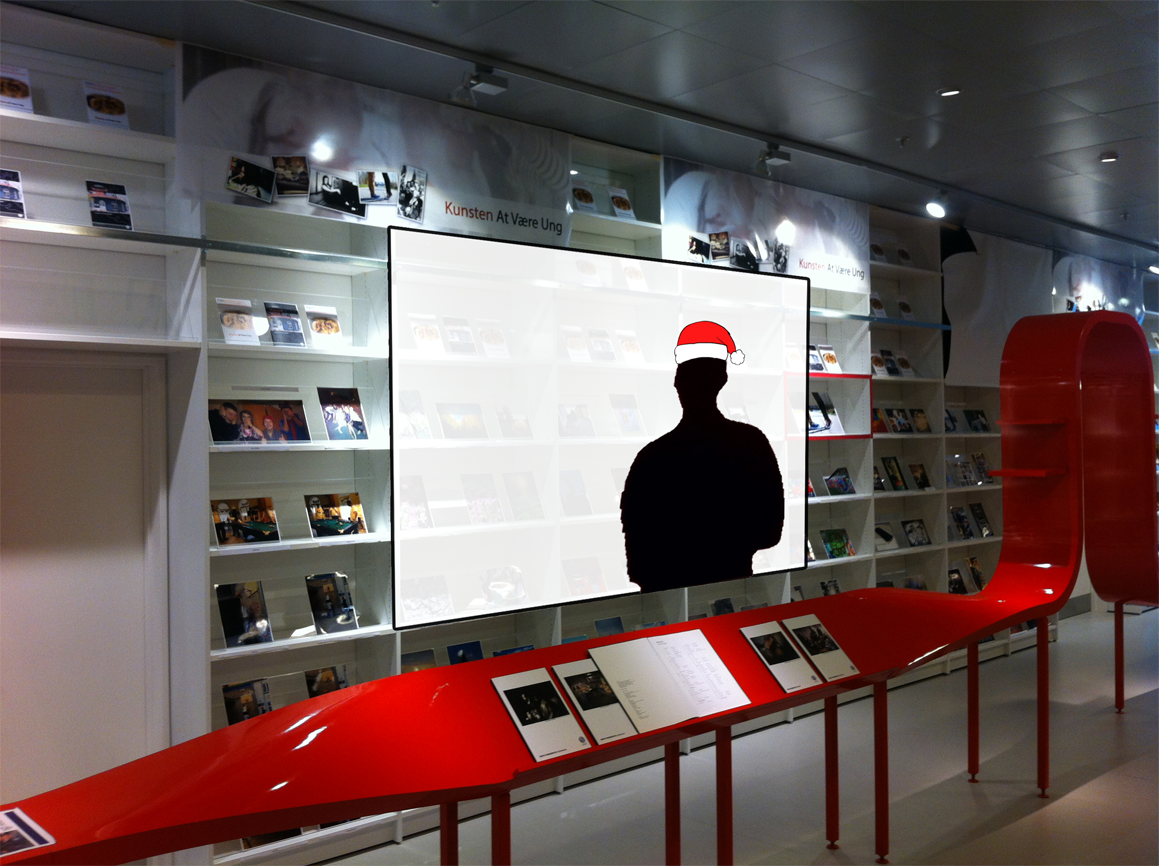
\includegraphics[width=1.00\textwidth]{Pictures/HjoerringLibrary/LocationJohannesHat.jpg}
\caption{Location a Hjørring Library}
\label{fig:concept_art}
\end{figure}
Figure \ref{fig:concept_art} illustrates the setup at the library. A canvas with the proportions 3*2.25 meters will be positioned directly on the bookshelves seen in the background of the picture.

\subsection{The initial goal}

\section{Technical Point of view}
The basic idea is to have a canvas on which the shade of the person is projected together with the Christmas hat added to the top of the head. For that some tools are needed:

\begin{itemize}
\item A web cam to gather input about people trespassing
\item A laptop to run the program code
\item A projector to display the output from the computer
\item A canvas on which the output is projected on
\item Controllable lights/light conditions
\item Power, cables etc.
\end{itemize}

Together with a projector capable of projecting a relative huge output 3*2.25 meters, the laptop running the program code will also be connected to a web cam. A canvas in above-mentioned size will have to be made and placed on-top of the book-shelves illustrated on figure 1.1.

\subsection{Ground zero}
The first step into developing some usable software, was to write some scrappy code that would run and produce a measurable output. This was done by dividing the entire group consisting of 6 people into 2 smaller groups of 3 people, to come up with a solution on how to produce a segmentation of the video input. A competition within the group turned up to create the best program code in 3 days to be presented. And so the "winner's" code or parts from both projects would be incorporated in a testable file.\\
At the end of the week 2 programs were ready to be tested. Both programs were able to do same things, only the code differed. Some of the techniques used were: Median filtering, morphology(opening/closing), background subtraction, conversion from a colored image to a gray-scale image and most important a first draft of the BLOB analysis, needed to analyse the shape of the head where the Christmas hat is to be placed.\\
One team did however create some custom made structures so that all would be able to include their own functions in the program without interfering with areas. Therefore it was decided to use that program to implement the different functions.

\subsection{Running the first test}


\subsection{Github}
bla bla bla..

\subsection{The equipment} 
modified to collect inferred lightning. This works by having some lamps that projects inferred light, that is "collectable" by the camera. We 

\section{Ultimate goal}
Prototype ready for 1st of December\\
Easy or almost self-maintained
\section{Problem Statement}
      
\textbf{We want an interesting expose at the library that you can enjoy at two different levels. 1) You can walk by and it's funny and 2) you can interact and bring your friends.}\\
\textbf{Easy or almost self-maintained.}

\section{This is awesome}
Yep yep

\begin{figure}[htbp]
\centering
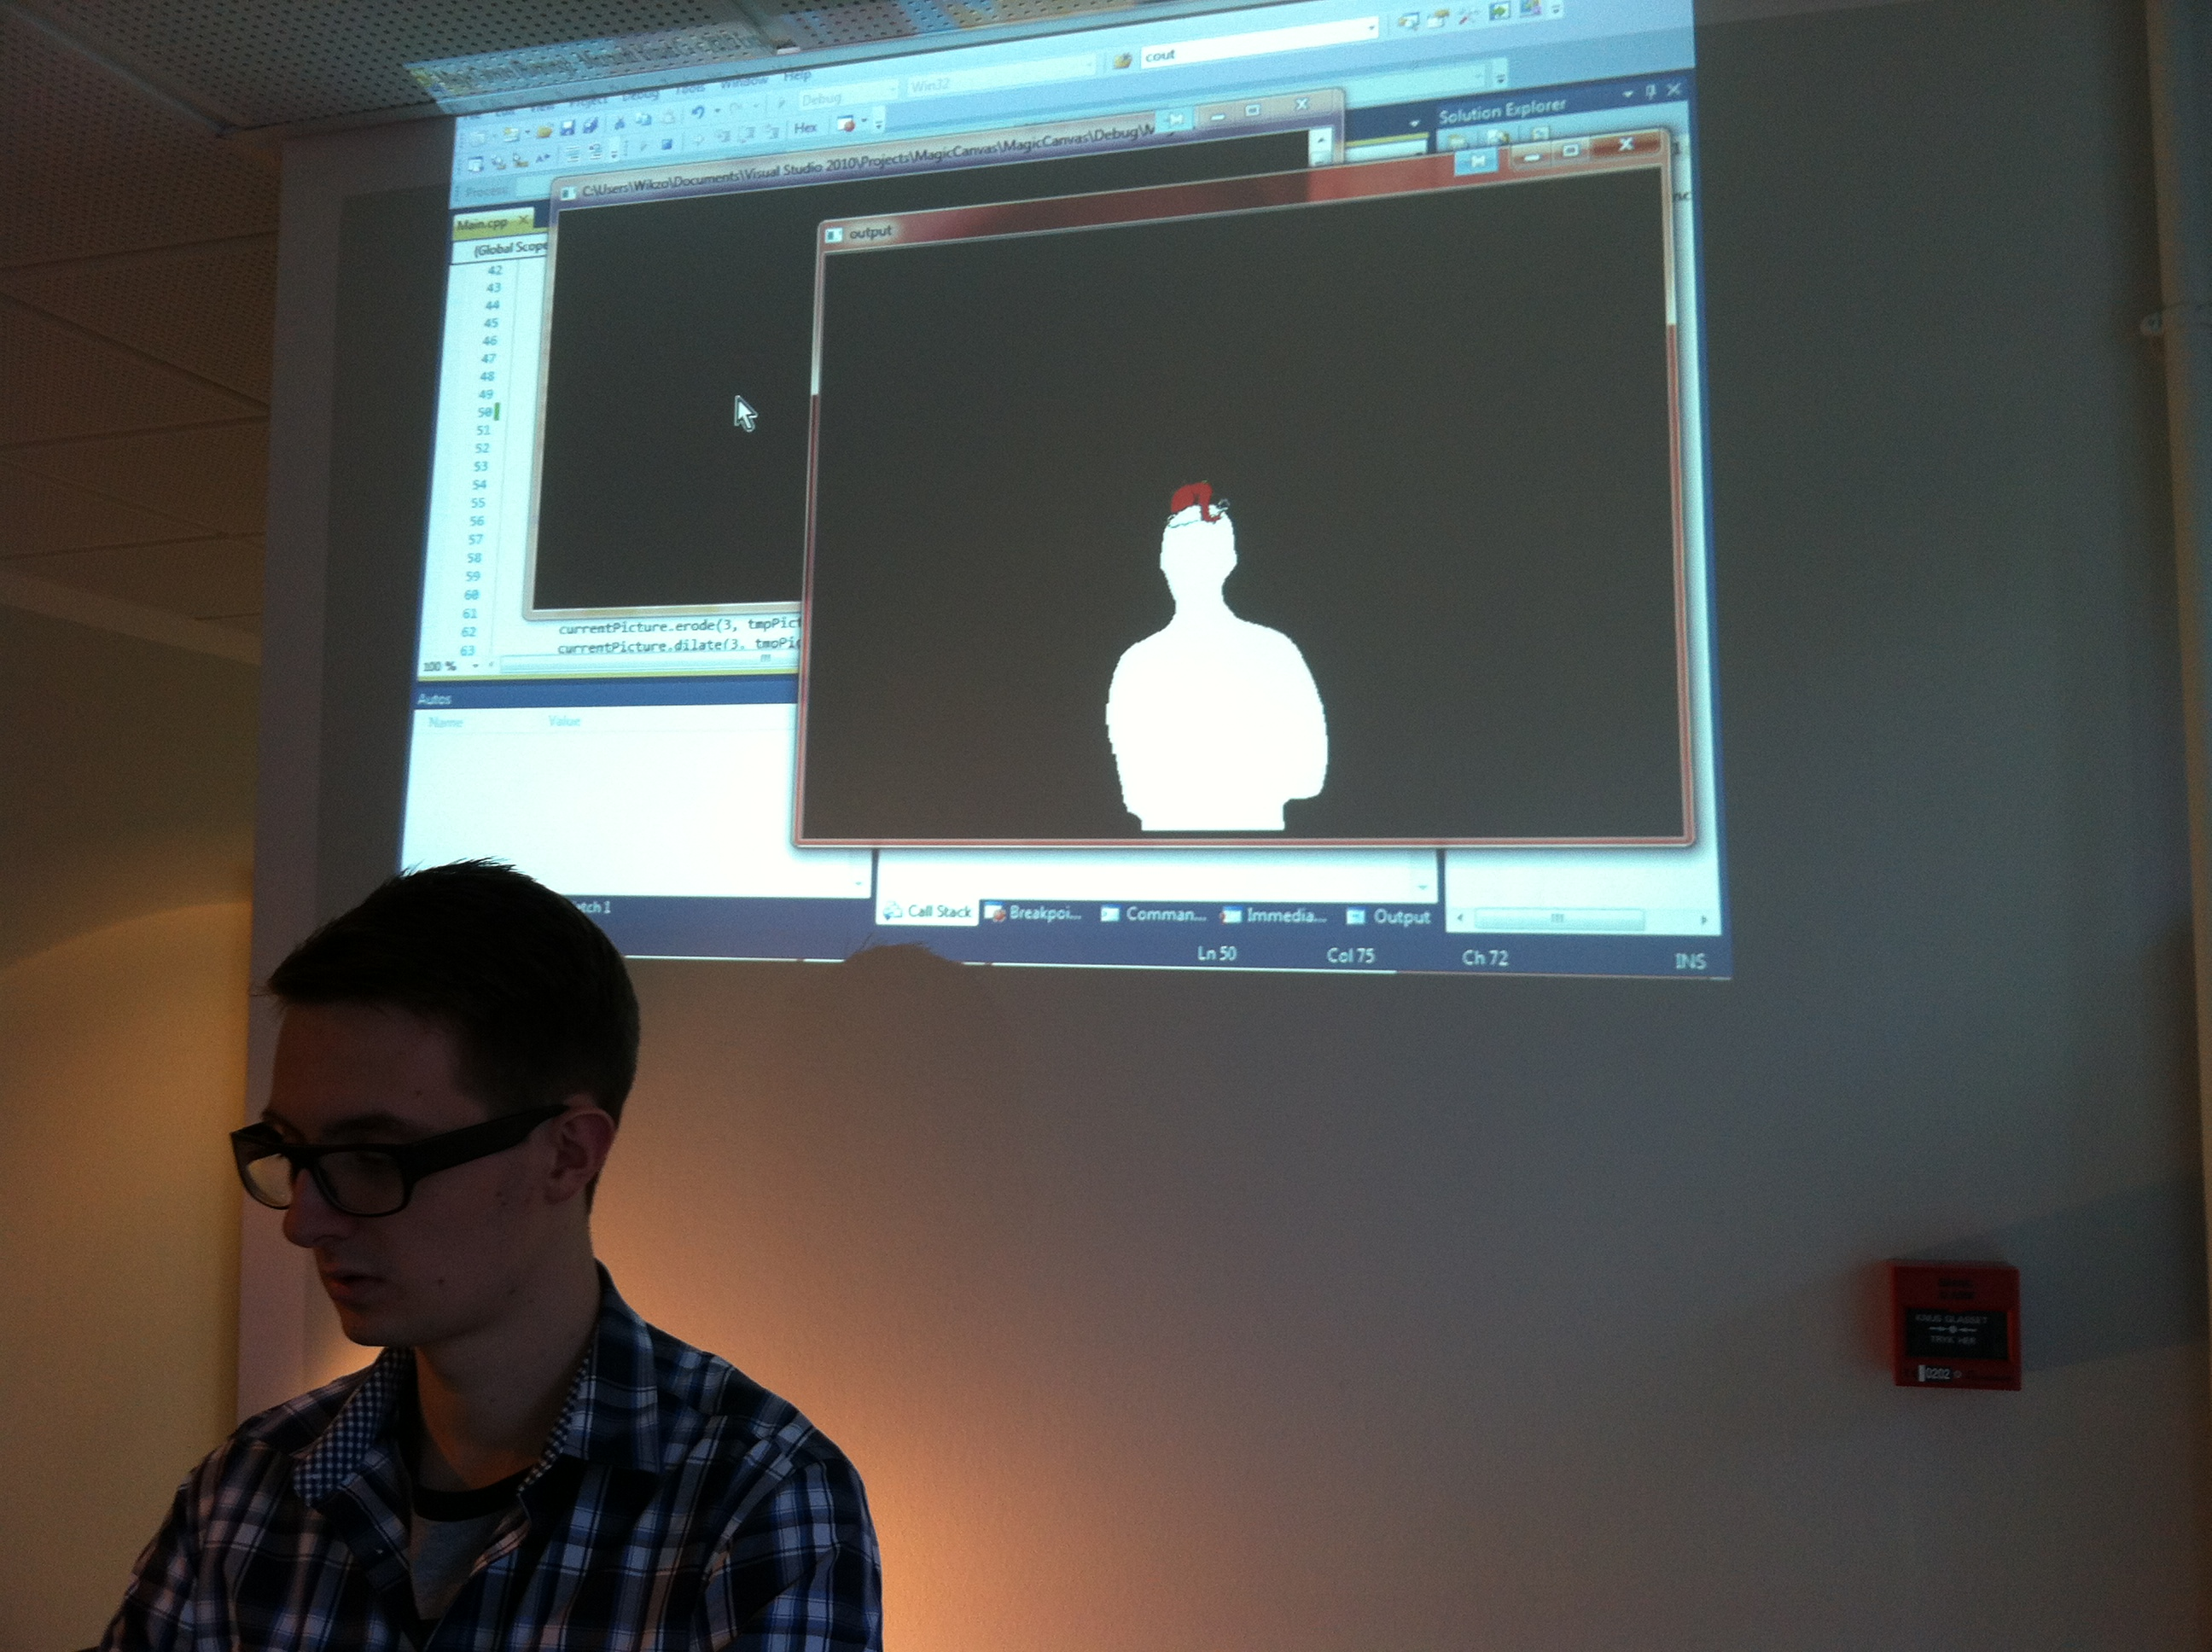
\includegraphics[width=1.00\textwidth]{Pictures/Test/IMG_1477.jpg}
\caption{Picture from Testing the Inferred Camera}
\label{fig:Picture from Testing the Inferred Camera}
\end{figure}

\subsection{Subway is good}
Nah...
